\documentclass{article}
\newcommand\tab[1][1cm]{\hspace*{#1}}
\usepackage[margin=60pt]{geometry}
\usepackage{hyperref}
\usepackage{makeidx}
\usepackage{graphicx}
\graphicspath{{./res/}}
\makeindex
\begin{document}
\begin{titlepage}
   \vspace*{\stretch{1.0}}
   \begin{center}
      \Huge\textbf{Progetto di Reti Logiche}\\
      \vspace{5mm} %5mm vertical space
      \Large Prof. Gianluca Palermo - Anno 2019/2020\\
      \vspace{5mm} %5mm vertical space
      \large\textit{Rigutti Luca [codice persona: 10558383]}
      \linebreak
      \large\textit{Tortorelli Giuseppe [codice persona: 10582962]}
   \end{center}
   \vspace*{\stretch{2.0}}
\end{titlepage}
\printindex

\tableofcontents
\pagebreak

\section{Introduzione}
\subsection{Scopo del progetto}
Il progetto di reti logiche dell'anno accademico 2019-2020 si basa sul metodo di codifica a bassa dissipazione di potenza detto "Working Zone".
Il metodo Working Zone lavora sul \textit{Bus} Indirizzi e si usa per codificare il valore di un indirizzo nel caso questo appartenga a certi intervalli noti: le working-zone. Ci possono essere multiple working-zone, ognuna delle quali parte da un indirizzo base e si estende per una dimensione fissa.
\subsection{Specifiche generali}
Vengono fornite otto working-zone e l'indirizzo da codificare. Ogni working-zone parte dall'indirizzo base e si estende per una dimensione complessiva di quattro indirizzi (incluso quello base).\\Si possono presentare due casi:
\begin{enumerate}
\item\textbf{Indirizzo non presente in nessuna working-zone}\\
In questo caso l'indirizzo codificato da restituire in \textit{output} è così formato:
\begin{center}
\textbf{WZ\_BIT} \& \textbf{ADDR}
\end{center}
\begin{itemize}
\item\textbf{WZ\_BIT}: è il \textit{\textit{bit}} che indica se l'indirizzo appartiene o meno a qualche working-zone ed in questo caso vale 0.
\item\textbf{ADDR}: è l'indirizzo originale fornito in \textit{input}.
\end{itemize}
\item\textbf{Indirizzo presente in una working-zone}\\
In questo caso l'indirizzo codificato da restituire in output è così formato:
\begin{center}
\textbf{WZ\_BIT} \& \textbf{WZ\_NUM} \& \textbf{WZ\_OFFSET}
\end{center}
\begin{itemize}
\item\textbf{WZ\_BIT}: è il \textit{\textit{bit}} che indica se l'indirizzo appartiene o meno a qualche working-zone ed in questo caso vale 1.
\item\textbf{WZ\_NUM}: è il numero della working-zone a cui l'indirizzo appartiene.
\item\textbf{WZ\_OFFSET}: è l'\textit{offset} tra l'indirizzo base della working-zone e l'indirizzo da codificare.
\end{itemize}
\end{enumerate}
L'indirizzo da codificare è espresso su 7 \textit{\textit{bit}}, in modo tale da rappresentare tutti i valori che vanno da 0 a 127. Gli indirizzi base delle otto working-zone e l'indirizzo codificato sono espressi su 8 \textit{\textit{bit}}.\\
WZ\_NUM è espresso su 3 \textit{\textit{bit}} per rappresentare gli otto indirizzi, quindi WZ\_OFFSET su 4 \textit{\textit{bit}}.\\
In particolare WZ\_OFFSET è codificato \textit{one-hot} così come segue:
\begin{itemize}
\item WZ\_OFFSET = 0 è codificato come 0001;
\item WZ\_OFFSET = 1 è codificato come 0010;
\item WZ\_OFFSET = 2 è codificato come 0100;
\item WZ\_OFFSET = 3 è codificato come 1000;
\end{itemize}
\pagebreak
\subsection{Interfaccia del componente}
{\fontfamily{qcr}\selectfont
entity poject\_reti\_logiche is\\
\tab port (\\
\tab\tab i\_clk\hspace*{1,5cm} : in std\_logic;\\
\tab\tab i\_start\hspace*{1,1cm} : in std\_logic;\\
\tab\tab i\_rst\hspace*{1,5cm} : in std\_logic;\\
\tab\tab i\_data\hspace*{1,3cm} : in std\_logic\_vector(7 downto 0);\\
\tab\tab o\_address\hspace*{0,7cm} : out std\_logic\_vector(15 downto 0);\\
\tab\tab o\_done\hspace*{1,3cm} : out std\_logic;\\
\tab\tab o\_en\hspace*{1,7cm} : out std\_logic;\\
\tab\tab o\_we\hspace*{1,7cm} : out std\_logic;\\
\tab\tab o\_data\hspace*{1,3cm} : out std\_logic\_vector(7 downto 0)\\
\tab );\\
end project\_reti\_logiche;
}
\begin{itemize}
\vspace{5mm} %5mm vertical space
\item i\_clk è il segnale di CLOCK;
\item i\_start è il segnale di START;
\item i\_rst è il segnale di RESET;
\item i\_data è il segnale che arriva dalla memoria in seguto ad una richiesta di lettura;
\item o\_address è il segnale di uscita che manda l'indirizzo alla memoria;
\item o\_done è il segnale di uscita che comunica la fine dell'elaborazione
\item o\_en è il segnale di ENABLE da mandare alla memoria per abilitare le operazioni sulla memoria
\item o\_we è il segnale di WRITE ENABLE da mandare alla memoria per abilitare la scrittura, quando in concomitanza con il segnale o\_en attivo
\item o\_data è il segnale di uscita che invia alla memoria l'indirizzo codificato
\end{itemize}
\pagebreak
\subsection{Dati e descrizione memoria}
I dati, ciascuno di dimensione 8 \textit{bit} (ADDR è esteso con uno 0 in posizione più significativa), sono memorizzati in una memoria RAM di sedici celle con indirizzamento al \textit{byte}:
\begin{itemize}
\item Le cella di indirizzi dallo 0 al 7 contengono gli indirizzi base delle otto working-zone;
\item La cella di indirizzo 8 contiene l'indirizzo da codificare;
\item La cella di indirizzo 9 contiene l'indirizzo codificato che viene fornito in \textit{output};
\item Le restanti celle sono inutilizzate;
\end{itemize}
\begin{figure}[h]
    \centering
    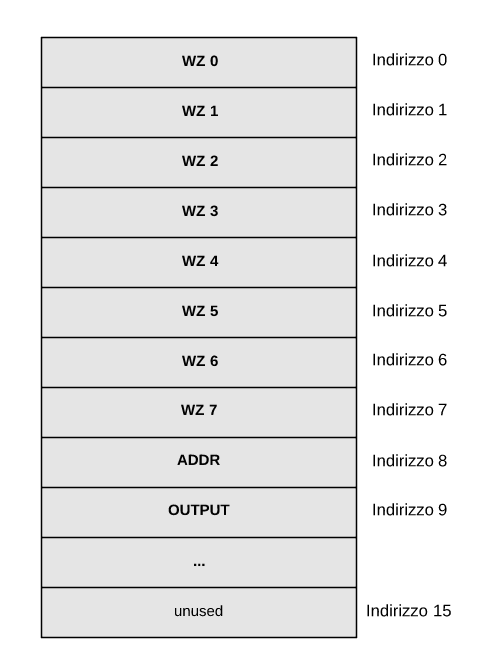
\includegraphics[width=0.5\textwidth]{memoria}
    \caption{schema della memoria}
\end{figure}
\pagebreak
\section{Design}
L'esecuzione inzia con un segnale di {\fontfamily{qcr}\selectfont i\_rst} posto a 1. Dopo l'abbassamento di {\fontfamily{qcr}\selectfont i\_rst}, si attende che {\fontfamily{qcr}\selectfont i\_start} diventi 1. Quest'ultimo rimmarrà alto fintanto che il segnale {\fontfamily{qcr}\selectfont o\_done} è basso. Quindi, dopo aver portato a 1 il segnale {\fontfamily{qcr}\selectfont o\_en}, si inizia con il prendere i dati dalla memoria.\\Successivamente si abilita il segnale di scrittura ({\fontfamily{qcr}\selectfont o\_we}) e si cerca la working-zone corrispondente all'indirizzo da codificare. A seconda che la working-zone venga trovata o meno, si scrive sul segnale {\fontfamily{qcr}\selectfont o\_data} l'indirizzo codificato nella maniera opportuna. Conclusa questa fase, si porta il segnale {\fontfamily{qcr}\selectfont o\_done} a 1 per indicare di aver finito con l'esecuzione e in modo tale da poter far scendere prima {\fontfamily{qcr}\selectfont i\_start} e di conseguenza ancora {\fontfamily{qcr}\selectfont o\_done}. Quindi la macchina si pone in attesa di un nuovo segnale di inizio o di reset con la differenza che nel primo caso si procede a leggere la memoria solo nella posizione corrispondente all'indirizzo da codificare.\\
L'implementazione è stata sviluppata tramite un'unica architettura di tipo \textit{Behavioral}. Di seguito sono illustrati i vari segnali interni utilizzati:\\\\
{\fontfamily{qcr}\selectfont
signal wz0 : std\_logic\_vector(7 downto 0);\\
signal wz1 : std\_logic\_vector(7 downto 0);\\
signal wz2 : std\_logic\_vector(7 downto 0);\\
signal wz3 : std\_logic\_vector(7 downto 0);\\
signal wz4 : std\_logic\_vector(7 downto 0);\\
signal wz5 : std\_logic\_vector(7 downto 0);\\
signal wz6 : std\_logic\_vector(7 downto 0);\\
signal wz7 : std\_logic\_vector(7 downto 0);\\
signal addr : std\_logic\_vector(7 downto 0);\\
signal en\_status : std\_logic;\\
signal we\_status : std\_logic;\\
signal wz\_found : std\_logic;\\
signal encode\_status : std\_logic;\\
signal tmp\_o\_data : std\_logic\_vector( 7 downto 0);\\
signal mem\_counter : integer;\\
signal status : integer;\\
}
\begin{itemize}
\item {\fontfamily{qcr}\selectfont wz0} : è utilizzato per memorizzare l'indirizzo base della prima working-zone;
\item {\fontfamily{qcr}\selectfont wz1} : è utilizzato per memorizzare l'indirizzo base della seconda working-zone;
\item {\fontfamily{qcr}\selectfont wz2} : è utilizzato per memorizzare l'indirizzo base della terza working-zone;
\item {\fontfamily{qcr}\selectfont wz3} : è utilizzato per memorizzare l'indirizzo base della quarta working-zone;
\item {\fontfamily{qcr}\selectfont wz4} : è utilizzato per memorizzare l'indirizzo base della quinta working-zone;
\item {\fontfamily{qcr}\selectfont wz5} : è utilizzato per memorizzare l'indirizzo base della sensta working-zone;
\item {\fontfamily{qcr}\selectfont wz6} : è utilizzato per memorizzare l'indirizzo base della settima working-zone;
\item {\fontfamily{qcr}\selectfont wz7} : è utilizzato per memorizzare l'indirizzo base della ottava working-zone;
\item {\fontfamily{qcr}\selectfont addr} : è utilizzato per memorizzare l'indirizzo da codificare;
\item {\fontfamily{qcr}\selectfont en\_status} : è utilizzato per controllare il valore di {\fontfamily{qcr}\selectfont o\_en};
\item {\fontfamily{qcr}\selectfont wn\_status} : è utilizzato per controllare il valore di {\fontfamily{qcr}\selectfont o\_we};
\item {\fontfamily{qcr}\selectfont wz\_found} : è utilizzato per controllare se l'indirizzo è stato trovato in una delle working-zone;
\item {\fontfamily{qcr}\selectfont encode\_status} : è utilizzato per controllare la fare si codifica;
\item {\fontfamily{qcr}\selectfont tmp\_o\_data} : è utilizzato per memorizzare un valore temporaneo dell'indirizzo codificato;
\item {\fontfamily{qcr}\selectfont mem\_counter} : è utilizzato per realizzare il contatore che legge i valori dalla memoria;
\item {\fontfamily{qcr}\selectfont status} : è utilizzato per distinguere le varie fasi di esecuzione della macchina;
\end{itemize}
\pagebreak
\subsection{Stati della macchina}
Le principali fasi di esecuzione sono scandite dal segnale {\fontfamily{qcr}\selectfont status}. Di seguito la descrizione precisa degli stati più interessanti della macchina.
\begin{figure}[h]
    \centering
    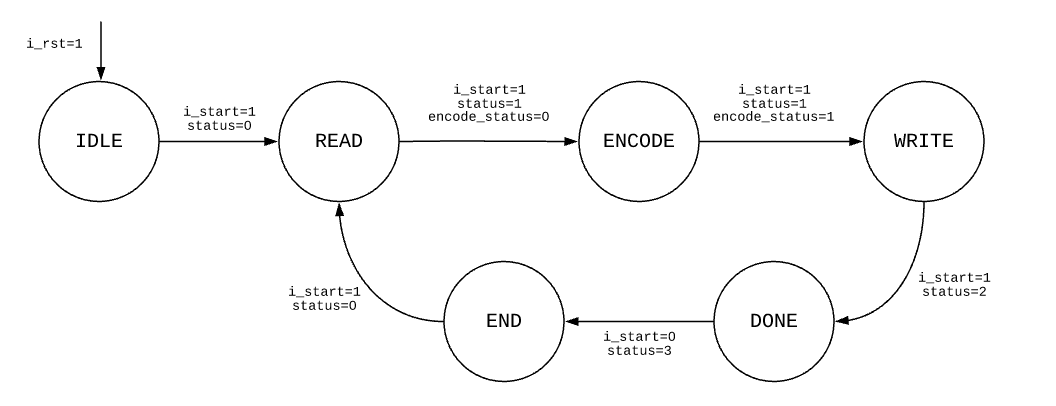
\includegraphics[width=0.8\textwidth]{fsa}
    \caption{diagramma degli stati}
\end{figure}
\subsubsection{IDLE: {\fontfamily{qcr}\selectfont i\_rst} = 0}
Lo stato si \textit{reset} nel quale vengono inizializzati i segnali.
\subsubsection{READ: {\fontfamily{qcr}\selectfont i\_start} = 1 e {\fontfamily{qcr}\selectfont status} = 0}
Dopo un ciclo di \textit{clock} utile per attivare la lettura tramite i segnali {\fontfamily{qcr}\selectfont en\_status} e {\fontfamily{qcr}\selectfont o\_en}, inizia il contatore che legge i dati dalla memoria: ogni due cicli di \textit{clock} viene posto in {\fontfamily{qcr}\selectfont o\_address} l'indirizzo della memoria che contiene il valore che si vuole leggere al ciclo successivo. La scelta di leggere un dato ogni due cicli è stata presa al fine di evitare sfasamenti sulla lettura dei dati a causa di eventuali ritardi. Va precisato che se gli eventuali ritardi superano il periodo del clock la soluzione adottata non risulta efficace, ma dal momento che non è fornito alcun modo per verificare se il dato richiesto è stato effettivamente ricevuto, abbiamo assunto che tali ritardi siano frutto di un funzionamento non contemplato della macchina [usare solo come appunto per chiedere all'esercitatore].
\subsubsection{ENCODE: {\fontfamily{qcr}\selectfont i\_start} = 1, {\fontfamily{qcr}\selectfont status} = 1 e {\fontfamily{qcr}\selectfont encode\_status} = 0}
Dopo un ciclo di \textit{clock} utile per attivare la scrittura tramite i segnali {\fontfamily{qcr}\selectfont we\_status} e {\fontfamily{qcr}\selectfont o\_we}, inizia la fase di codifica. Viene confrontato l'indirizzo da codificare con ogni set di working-zone parallelamente e nel caso venga trovata una corrispondenza si scrive l'indirizzo codificato in {\fontfamily{qcr}\selectfont temp\_o\_data}. Il segnale {\fontfamily{qcr}\selectfont wz\_found} serve per discriminare se la working-zone è stata trovata o meno.
\subsubsection{WRITE: {\fontfamily{qcr}\selectfont i\_start} = 1, {\fontfamily{qcr}\selectfont status} = 1 e {\fontfamily{qcr}\selectfont encode\_status} = 1}
Questo è lo stato in cui viene scritto il risultato nella memoria. Grazie al segnale {\fontfamily{qcr}\selectfont wz\_found} è possibile scrivere l'indirizzo codificato nella maniera opportuna.
\subsubsection{DONE: {\fontfamily{qcr}\selectfont i\_start} = 1 e {\fontfamily{qcr}\selectfont status} = 2}
Finita l'elaborazione, si settano i vari segnali ai valori opportuni e si alza il segnale di {\fontfamily{qcr}\selectfont o\_done} per notificare che l'esecuzione è stata completata.
\subsubsection{END: {\fontfamily{qcr}\selectfont i\_start} = 0 e {\fontfamily{qcr}\selectfont status} = 3}
{\fontfamily{qcr}\selectfont i\_start} è tornato a 0 quindi si riabbassa anche {\fontfamily{qcr}\selectfont o\_done}.\\
I segnali {\fontfamily{qcr}\selectfont mem\_counter} e {\fontfamily{qcr}\selectfont o\_address} vengono settati in maniera tale da entrare nel ciclo di conteggio (stato READ) nel momento della lettura dell'indirizzo da codificae. Questo perchè gli indirizzi delle working-zone non cambiano tra un segnale di start e un'altro ma solamente quando viene resettata la macchina.
\pagebreak
\section{Risultati dei test}
\section{Conclusione}
\subsection{Risultati della sintesi}
Il componente sintetizzato supera correttamente tutti i test specificati nelle tre simulazioni: \textit{Behavioral}, \\\textit{Post-Synthesis Functional} e \textit{Post-Synthesis Timing}. Inoltre tutti i test restituiscono esito positivo sia in \textit{Pre-Synthesis} che in \textit{Post-Synthesis}, con un periodo di \textit{clock} fino a 1[ns].\\ Di seguito lo schema del circuito sintetizzato.
\begin{figure}[h]
    \centering
    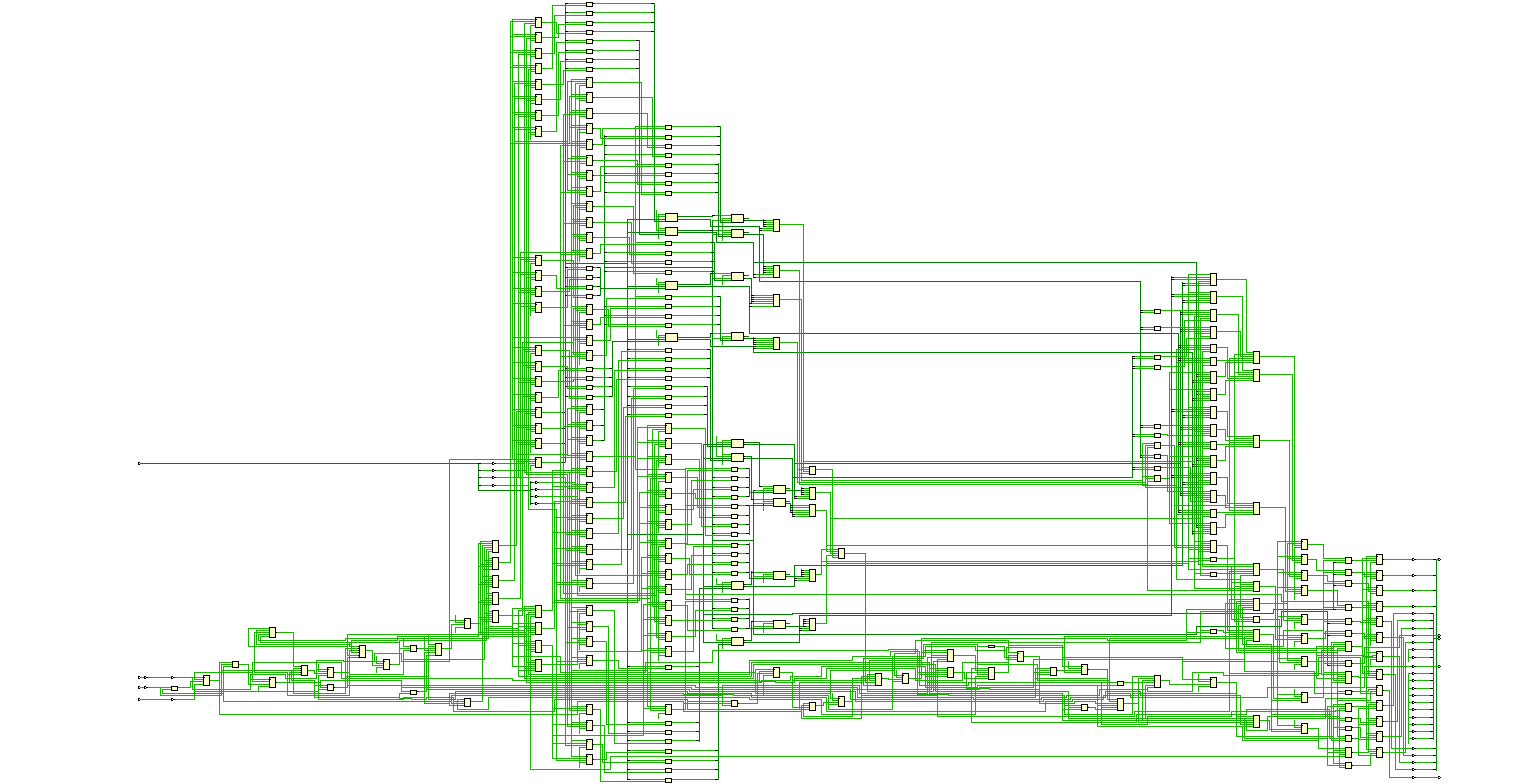
\includegraphics[width=1\textwidth]{schema}
    
\includegraphics[width=1\textwidth]{spazio}
    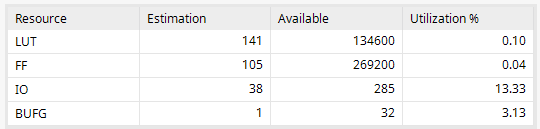
\includegraphics[width=0.7\textwidth]{utilizzo}
    \caption{schema del circuito e tabella di utilizzo}
\end{figure}
\end{document}
